To achieve our objective of building a spanning tree that minimizes the distances between all
connected pair of nodes in the original graph, we rely on a particular subgraph structure, namely
the star.  We therefore introduce two algorithmic primitives: \extractStar{}, which partition a
graph $G$ into a set of disjoint stars; and \collapseStar{}, which selects edges from $E$ to
assemble these stars into a new, smaller graph. Given a graph topology $G_0=(V_0, E_0)$ and assuming
for simplicity that $G_0$ consists of a single connected component,\footnote{For we can otherwise
run our algorithm in parallel on each connected components of $G_0$.} the \gtx{} algorithm
repeatedly applies these two primitives to produce a sequence of graphs $\{G_t\}_{t=0}^K$ of
decreasing size, until $G_K$ is made of a single node. All the edges selected while reaching
this stage then form the spanning tree we were looking for.
% [from a CMU NIPS submission http://www.stat.cmu.edu/~arinaldo/papers/mutualfriends.pdf] We
% consider Mutual-Friends to be *an algorithmic primitive*, by which we mean a kind of subroutine for
% a more complicated function that iterates Mutual-Friends, similarly to [5].

In the following, we provide a more precise description of our two primitives and analyze their
complexity. Then we state formally the complete \gtx{} algorithm, prove its termination and
correctness, and show a detailed example of its execution.  Finally, we study its properties, such
as the number of iterations needed to finish and the stretch of the resulting tree.

\paragraph{\extractStar{}}\label{par:extractstar}%
\extractStar{} takes as input a graph $G_t=(V_t, E_t)$.
While the nodeset $V_t$ is not exhausted, it repeatedly samples a
node $c_i$, creates a star $S_i^t$ with $c_i$ at its center and the neighbors of $c_i$ on the
periphery, removes all the nodes of $S_i^t$ from
$V_t$ and all the edges incident to $S_i^t$ from $E_t$, and finally decrements accordingly the
degree of the 2-hop neighbors of $c_i$ (see \autoref{fig:gtx_star_simple} for a visual
representation of this notation).
Upon completion, it returns a list of stars,
the set of all the edges within a star,
and a map (or associative array) that associates each node of $V_t$ to the index of the
unique star it belongs to.
According to the definition of \textcite{HashTableBook08}, an associative array is an abstract data
type composed of a collection of (key, value) pairs, such that each possible key appears at most
once in the collection. It efficiently supports the addition, removal and modification of a pair, as
well as the lookup of a value associated with a particular key.
\begin{marginfigure}
  \centering
  \includegraphics[height=0.15\textheight]{assets/tikz/gtx_star_tikz.pdf}
  \caption[A sample star]{A sample star created during the \tth{} collapse level. The black node
    % \tikz{\node[vertex,rare] {$c_i$};}
    is the center $c_i$ of the star $S_i^t$, which is also made of the four light gray peripheral nodes
  % \tikz{\node[vertex,medium] {$p_1$};} to \tikz{\node[vertex,medium] {$p_4$};}
  as well as the solid edges. The 2-hops neighbors of $c_i$ are the white nodes
  % \tikz{\node[vertex] {$h_1$};} to \tikz{\node[vertex] {$h_3$};}
  $h_1$ to $h_3$, whose degree will decrease once $S_i^t$ is removed from $G_t$.}
  \label{fig:gtx_star_simple}
\end{marginfigure}

As showed in the following pseudo code\footnote{Note that for
clarity, we removed some bookkeeping code in all listings, mainly the part related to maintaining
mapping between nodes at different collapse level. However, the full python implementation
is available at \url{https://github.com/daureg/magnet/blob/master/veverica/new_galaxy.py\#L27}.}, we
sample centers by choosing the node with the current highest degree, with ties broken
arbitrarily.\footnote{We also consider more involved heuristics but, in the interest of simplicity,
they are presented later~\vpageref{ssec:gtx_center_choice}.} This is achieved efficiently by
maintaining a max-priority queue $Q$, initially containing all the nodes of $V_t$. The priority of a
node is its current degree and we equip $Q$ with two standard operations described
by~\textcite[section 6.5]{CormenAlgo09}: \textsc{Extract-Max}$(Q)$ removes and returns the
node of $Q$ with the largest degree and \textsc{Decrease-Key}$(Q$, $u$, $\Delta)$ decrements
the degree of the node $u$ by an amount $\Delta$.
We also assume that $G$ is the adjacency list of the graph, so that $G[u]$ is the set of neighbors of
$u$, \ie{} $G[u] \equiv \mathcal{N}(u)$. Finally $membership$ is a map and we
define the \textsc{Star} function, which creates a star given a center $c$, a list $periphery$ of
peripheral nodes, and a star index $i$. After creating the \ith{} star, for every node $u$ belonging
to that star, the \textsc{Star} function sets $membership[u] = i$.
\vspace{-\baselineskip}

\begin{center}
  \rule{\textwidth}{.3pt}
  \begin{algorithmic}[1]
    \Function{\extractStar{}}{$G_t=(V_t,E_t)$}
      \State Let $Q$ be the max-priority queue described above
      \State Let $remaining$ be a set of nodes, initially containing all the nodes in $V_t$
      \State Let $membership$ be an empty map
      \Let{$stars$}{$[]$}
      \Let{$inner\_edges$}{$\emptyset$}
      \While{$Q$ is not empty}
        \Let{$c$}{\Call{Extract-Max}{$Q$}}
        \If{$c$ not in $remaining$}
          \State \textbf{continue} \Comment{$c$ is part of an existing star so there is
          nothing to do}
        \EndIf
        \Let{$periphery$}{$G_t[c] \bigcap remaining$}
        \Let{$stars$}{$stars \bigcup \{$\Call{Star}{$c$, $periphery$, $|stars|$}\}}
        \Let{$inner\_edges$}{$inner\_edges \bigcup \{(c, p): p \in periphery\}$}
        \Let{$remaining$}{$remaining \setminus \left\{ \{c_i\} \cup periphery\right\}$}
        \For{$p$ in $periphery$}
          \For{$h$ in $G_t[p] \bigcap remaining$}
            \State \Call{Decrease-Key}{$Q$, $h$, $1$}
          \EndFor
        \EndFor
      \EndWhile
      \State \textbf{return} $stars$, $inner\_edges$, $membership$
    \EndFunction
  \end{algorithmic}
  \rule{\textwidth}{.3pt}
\end{center}

\begin{prop}
  For any connected graph $G=(V,E)$, \extractStar$(G)$ terminates in $O(|E|)$ time.
\end{prop}
\begin{proof}
\extractStar{} terminates because at each iteration of the while loop line 7, we remove one node
from $Q$ and never add any. Let us now analyze its complexity. We first build a priority queue of
all the nodes according to their degree (line 2), which requires $O(|V|)$ insertions into $Q$. Then
we execute $|V|$ iterations of the while loop. However, the main idea here is that we process each
node and each edge exactly once. We first find the center $c$ of the next star by extracting the
maximum of the queue (line 8) and testing if $c$ is still part of the graph, which happens $|V|$
time. Then we build the corresponding star (line 11--14). In total, we test the membership of $|V|$
nodes in line 11, $\textsc{Star}$ updates the $membership$ map $|V|$ times in line 12,
$inner\_edges$ consists of $|E|$ edges at most in line 13 and $remaining$ is only updated $|V|$
times in line 14. Finally, we decrease the priority (\ie{} the degree) of all nodes adjacent to the
new star (line 15--17). Each decrement is supported by a single edge, thus \textsc{Decrease-Keys} is
called at most $|E|$ times. Since all queue operations require constant time when using a Strict
Fibonacci Heap~\autocite{FibonacciHeaps12}, the complexity is $O(|E|+|V|)$, which is also $O(|E|)$
since $G$ is connected.
\end{proof}

\paragraph{\collapseStar{}}\label{par:collapsestar}%
The second primitive, \collapseStar{} takes as input the result of \extractStar{}, along with $E_t$
and an optional $\emph{eccentricity}$ array we will describe soon\marginpars{Actually, we could make
eccentricity the default behavior, which would simplify the pseudo code}. It builds a new graph $G_{t+1}$
where each star becomes a node and where there is a link between two nodes $s_1$ and $s_2$ if the nodes
making up $s_1$ and $s_2$ are connected in $E_t$.

\begin{center}
  \rule{\textwidth}{.3pt}
  \begin{algorithmic}[1]
    \Function{\collapseStar{}}{$E_t,\,membership,\,eccentricity$}
      \State Let $G_{t+1}$ be an empty graph
      \State Let $cross\_edges$ be a mapping from edges in $G_{t+1}$ to set of edges in $G_t$
      \ForAll{edge $(u, v)$ in \Call{Shuffle}{$E_t$}}
        \Let{$s_u,\,s_v$}{$membership[u]$, $membership[v]$}%
        \Comment{swap if needed so that $s_u < s_v$}
        \If{$s_u = s_v$}
          \State \textbf{continue}
        \EndIf
        \If{$eccentricity$ is not \textbf{null}}
          \Let{$cross\_edges[(s_u, s_v)]$}{$cross\_edges[(s_u, s_v)] \bigcup \{(u, v)\}$}
          % \State $cross\_edges[(s_u, s_v)].$\Call{Add}{$(u, v)$}
        \ElsIf{$(s_u, s_v)$ not in $cross\_edges$}
          \Let{$cross\_edges[(s_u, s_v)]$}{$\{(u, v)\}$}
          \State Add edge $(s_u, s_v)$ to $G_{t+1}$
        \EndIf
      \EndFor
      \If{$eccentricity$ is not \textbf{null}}
        \ForAll{$\Big(\underbrace{(s_u,s_v)}_{\text{key}},\,
          \underbrace{candidate\_edges}_{\text{value}}\Big)$
          in $cross\_edges.$\Call{Items}{$\,$}}
          \Let{$(u_0, v_0)$}{$\argmin_{(u,v)\in candidate\_edges} eccentricity[u]+eccentricity[v]$}
          \Let{$cross\_edges[(s_u, s_v)]$}{$\{(u_0, v_0)\}$}
          \State Add edge $(s_u, s_v)$ to $G_{t+1}$
        \EndFor
      \EndIf
      \State \textbf{return} $G_{t+1}$, $cross\_edges$
    \EndFunction
  \end{algorithmic}
  \rule{\textwidth}{.3pt}
\end{center}

For that, we first shuffle $E_t$ and iterate on it (line 4). When we find an edge whose endpoints
belong to two different stars not yet connected (line 10), we use that edge to connect these two
stars (line 11--12) This trivially takes $O(m)$ times.  A variant instead keeps track of all edges
connecting each pair of stars (line 9) to choose one that will best contribute to our low stretch
objective. Namely, when connecting two stars, we would prefer to join their centers rather than two
peripheral points. For that we maintain an eccentricity count for all of the nodes of the original
$G_0$, which is incremented by $1$ each time a node is chosen to be on the periphery of a
star.\footnote{We will discuss this construction in more details when describing the main \gtx{}
function since it takes place there.} For each pair of stars, we thus choose the edge across them
with minimal sum of its endpoints' eccentricity (line 15--17)\marginpars{Line 15 is actually a
simplification since the $eccentricity$ array is only defined for nodes in $V_0$ so when
\collapseStar{} is called on $G_3$ for instance, $u$ and $v$ are nodes of $V_3$ and we have to
retrieve the actual corresponding edge in $E_0$. Maybe I could simply add a HashMap from $E_t$ to
$E_0$ like in the python code…}. This only requires another pass over the edges, thus preserving the
$O(m)$ runtime.

\paragraph{Putting the pieces together}\label{par:full_gtx}%
\extractStar{} and \collapseStar{} are truly the core the of \gtx{} algorithm but to obtain our
final spanning tree, we need additional work, namely updating the eccentricity of the nodes of
$V_0$ and keeping track of each edge within and between stars along every contraction level.

\begin{algorithm}
  \caption{\gtx{}($G_0=(V_0,E_0)$) \label{alg:gtx}}
	\begin{algorithmic}[1]
    \State Let $eccentricity$ be an array of size $|V_0|$ initially all set to $0$
    \Let{$G_t$}{$G_0$}
    \Let{$inner\_edges\_seq$, $outer\_edges\_seq$}{$[]$, $[]$}
    \Repeat
      \Let{$stars$, $inner\_edges$, $membership$}{\Call{Extract-Stars}{$G_t$}}
      \State $inner\_edges\_seq$.\Call{Append}{$inner\_edges$}
      \State \Call{Update-Eccentricity}{$stars$, $eccentricity$, $original\_node$}
      \Let{$full\_membership$, $original\_node$}{\Call{Update-Nodes-Mapping}{$full\_membership$, $membership$}}
      \Let{$G_{t+1}$, $\!outer\_edges$}{\Call{Collapse-Stars}{$E_t \!\setminus\! inner\_edges$,
      $\!membership$, $\!eccentricity$}}
      \State $outer\_edges\_seq$.\Call{Append}{$outer\_edges$}
      \Let{$G_{t}$}{$G_{t+1}$}
    \Until{$|outer\_edges|>0$}
    \State \textbf{return} \Call{Assemble-Spanning-Trees}{$inner\_edges\_seq$, $outer\_edges\_seq$}
		\begin{center}
      \vspace{-.5\baselineskip}
			\rule{0.5\textwidth}{.2pt}
		\end{center}
    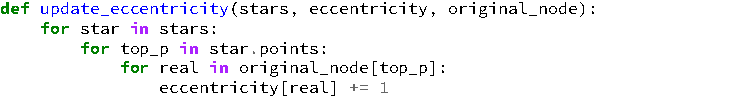
\includegraphics{assets/tmp-code/update_eccentricity.pdf}
    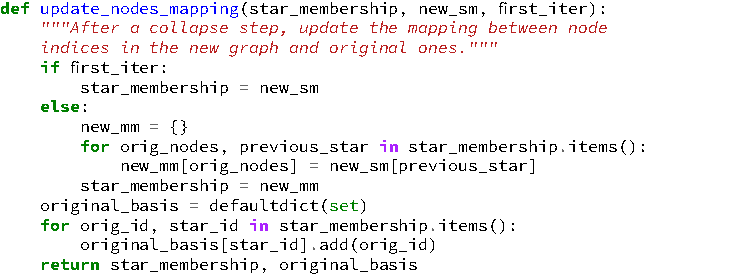
\includegraphics{assets/tmp-code/update_nodes_mapping.pdf}
    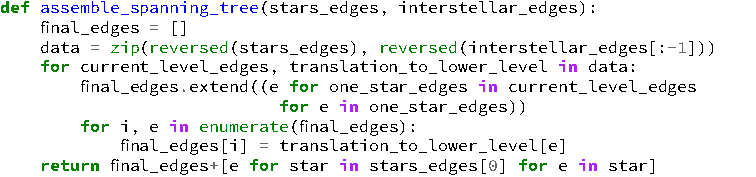
\includegraphics{assets/tmp-code/assemble_spanning_tree.pdf}
	\end{algorithmic}
\end{algorithm}

As described in \autoref{alg:gtx}, \marginpars{I didn't write pseudo code for the three helping functions but
instead put their verbatim python version. They are mostly plumbing code, the only interesting
aspect is their complexity.  \texttt{update\_centrality} and \texttt{update\_nodes\_mapping} takes
$O(n_0)$ time since they go through every node of the original graph. As for
\texttt{assemble\_spanning\_tree}, it goes again through every edges visited at every level of
contraction, meaning it's $O(Tm)$. However, we already visited those edges at least once so it only
adds a constant factor $2$ in the overall complexity of the \gtx{} algorithm.}
at every collapse level, we first extract stars from the current graph (line 5), then
update the eccentricity and nodes mapping (lines 7--8) and finally collapse the graph (line 9) We
perform these operations until there are no edge connecting stars anymore. At this point, we revisit
every outer edges to form the spanning tree (line 13). Because the main loop does not perform any
work besides calling other function, assuming there are T collapse steps, the complexity of \gtx{}
is $O(T(m+n)) = O(Tm)$.

Later we hope to found an upper bound of $T$ in terms of $m$, and also to refine the analysis to
leverage the fact that $\sum_{t=0}^T |E_t|$ is significantly smaller than $Tm$. For now, let us
prove the termination of \gtx{} by observing that, assuming $|E_t|>0$, $|E_{t+1}| < |E_t|$ since
at least two nodes in $G_t$ are connected and will therefore form a star, which will remove all the
inner edges of that star. As for the fact that we get a tree, note that a star is a tree, therefore
a star of star is a tree, and so on.\Todo{make the two arguments about \gtx{} correctness more
formal, and also explain that since all nodes are part of the ultimate star, this tree is a spanning
one. Motivate the name of \gtx{}.}

\paragraph{Exemple of \gtx{}}
\label{par:exemple_of_gtx}

We illustrate the operation of the \gtx{} algorithm on a small (and somewhat contrived) example.
Let us start with the initial graph $G_0$ depicted in \autoref{fig:gtx_eccentricity}
\vpageref{fig:gtx_eccentricity} and initialize
the eccentricity of all nodes to $0$. When running \extractStar{}, we see that the maximum degree is
$4$, achieved at nodes $\{1, 6, 11, 16, 21, 26, 31, 36, 41\}$. For the sake of simplicity, assume
nodes are picked according to their index. First, node $1$ forms the star $\starone{1}$ with
peripheral nodes $2$, $3$, $4$ and $5$. This increments the eccentricity of those peripheral nodes
by $1$. Then node $6$ forms its star $\starone{2}$ with $7$, $8$, $9$ and $10$. The process
continues until node $41$ is chosen to be the center of star $\starone{9}$, at which point the
max-priority queue has been exhausted and \extractStar{} finishes.

\begin{figure}[htbp]
  \centering
  \includegraphics[width=0.78\linewidth]{tikz/gtx_eccentricity_tikz.pdf}
  \caption[The hierarchical structure of stars created by \gtx{}]{%
    The execution of the \gtx{} algorithm. The original graph is made of the solid and dashed edges
    connecting the nodes labeled by their index. Edges forming the final spanning tree are solid
    while the others are dashed. Their colors indicate at which iteration they were chosen to be inside a
    star. The four shades of gray, from white to dark gray
    denote increasing node eccentricity (as computed at the end of the algorithm). The \ith{} star
    created during the \jth{} iteration of the algorithm is denoted $S_i^j$. Refer to the main text
    for the complete description of the execution.}
  \label{fig:gtx_eccentricity}
\end{figure}

\begin{figure}[bthp]
  \centering
  \begin{subfigure}[b]{0.47\textwidth}
    \centering
    \includegraphics[height=5cm]{tikz/gtx_run_level1_tikz}
    \caption{Resulting graph after the first iteration}\label{fig:gtx_run1}
  \end{subfigure}~
  \begin{subfigure}[b]{0.47\textwidth}
    \centering
    \includegraphics[height=2.2cm]{tikz/gtx_run_level2_tikz}
    \caption{Resulting graph after the second iteration}\label{fig:gtx_run2}
    \vspace{\baselineskip}
    \includegraphics[height=2.2cm]{tikz/gtx_run_level3_tikz}
    \caption{Resulting graph after the third iteration}\label{fig:gtx_run3}
  \end{subfigure}~
  \caption{The other iterations of \gtx{}}\label{fig:gtx_run}
\end{figure}

We then call \collapseStar{}. This will connect all possible pairs of star. For instance, the edge
between nodes $19$ and $29$ leads to the edge between $\starone{4}$ and $\starone{6}$. This is
actually the only possible edge between $\starone{4}$ and $\starone{6}$.  Consider on the other hand
the case of edges $(2, 6)$ and $(2, 9)$. They both connect $\starone{1}$ and $\starone{2}$. Yet at
this point of the algorithm, the eccentricity of node $2$ is $1$, the eccentricity of node $6$ is
$0$ and the eccentricity of node $9$ is $1$. The edge $(2, 6)$ has therefore the smallest total
eccentricity and is chosen to connect $\starone{1}$ and $\starone{2}$. The full result of the
\collapseStar{} procedure is $G_1$, which can be seen on \autoref{fig:gtx_run1}.

We now run \extractStar{} on $G_1$. Because all nodes have degree $2$, they could all be chosen to
be the center of a star yet we again they are picked according to their index and therefore we
choose $\starone{1}$ to be the center of the star $\startwo{1}$ with peripheral nodes $\starone{2}$
and $\starone{3}$. The original nodes belonging to those peripheral stars (nodes $4$ to $15$) have
their eccentricity incremented by $1$. The next node with highest degree in $G_1$ is now
$\starone{4}$, which forms a star with $\starone{5}$ and $\starone{6}$. This choice means that nodes
$21$ through $30$ have their eccentricity incremented by $1$. Finally, $\starone{7}$ forms the last
star with $\starone{8}$ and $\starone{9}$. Then \collapseStar{} connects the resulting three stars,
and this time there is only a single choice between each pair of stars, leading to the graph $G_2$
showed in \autoref{fig:gtx_run2}

The action of \extractStar{} on $G_2$ is quite simple, because there is only one star that can be
created, so let say we choose $\startwo{1}$ as its center, with $\startwo{2}$ and $\startwo{3}$ as
peripheral nodes. This increases the eccentricity of their underlying $G_0$ nodes by $1$ (namely
nodes $16$ to $45$). Because there is only one star $\starthree{1}$ left, \collapseStar{} returns
$G_3$ showed in \autoref{fig:gtx_run3} and an empty list of outer edges, meaning that the inner loop
of \gtx{} is finished and we can go through every edges we chose between stars at every level to
recover the final spanning tree, showed with solid edges in \autoref{fig:gtx_eccentricity}
\vpageref{fig:gtx_eccentricity}. For completeness, we can also look at the edges which are not part
of the spanning tree and therefore contribute to the stretch of the tree. In that case the average
stretch is $7$, as showed in \autoref{tab:gtx_example_stretch}.

\begin{table}[htpb]
  \centering
  \caption{Stretch of the example tree}
  \label{tab:gtx_example_stretch}
  \begin{tabulary}{\linewidth}{lLr}
    \toprule
    test edge & path in the tree & length \\
    \midrule
    $2,9$   & $2$--$6$--$9$                       & $2$ \\
    $3,12$  & $3$--$1$--$4$--$14$--$11$--$12$     & $6$ \\
    $13,29$ & $13$--$11$--$15$--$26$--$29$        & $4$ \\
    $20,24$ & $20$--$16$--$17$--$23$--$21$--$24$  & $5$ \\
    $25,42$ & $25$--$21$--$23$--$17$--$16$--$19$--$29$--$26$--$15$--$11$--$14$--$4$--$1$--$2$--$6$--$8$--$37$--$36$--$39$-- $32$--$31$--$35$--$43$--$41$--$45$ & $24$ \\
    $33,38$ & $33$--$31$--$32$--$39$--$36$--$38$  & $5$ \\
    $34,43$ & $34$--$31$--$35$--$43$              & $3$ \\
    \bottomrule
  \end{tabulary}
\end{table}

\paragraph{Number of iterations needed}\label{par:number_of_iteration}%

\textcolor{red}{\LARGE Draft}

A crucial quantity of the \gtx{} algorithm, both in terms of complexity and resulting stretch, is
the number of collapses $T$ needed before termination. While this is still elusive to express in the
general case, let us first look at some simple cases. For instance, a very sparse example of graph
is the line graph. While it is already a tree, let us look how the \gtx{} algorithm operates on it.
Say we have $n$ nodes in that line. There a star is made at most of three consecutive nodes. In the
worst case, centers will be chosen such that we have a succession of three and two nodes stars (as
in \autoref{fig:gtx_line_graph}).%
\begin{marginfigure}
  \centering
  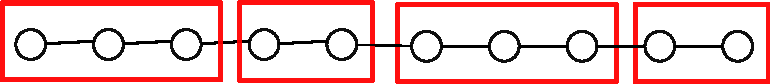
\includegraphics[width=0.9\linewidth]{assets/tmp-code/line_graph.pdf}
  \caption{A line graph with stars in red}
  \label{fig:gtx_line_graph}
\end{marginfigure}
This will results in $\nicefrac{2n}{5}$ stars, which is less than half of $n$ and because in that
case $n\approx m$, \gtx{} will finish after $O(\log m)$ iterations. Note that a barbell graph (two
cliques connected by a line) would require a number of iterations proportional to the length of that
central line, despite having many more edges. This suggests unsurprisingly that the diameter of the graph
could be a good parameter to quantify the number of iteration needed. Indeed, take a tree a consider
the length $p$ of its longest path from the root to a leaf. By a similar argument as the one used in
the line case, it seems \gtx{} will terminate after $O(\log p)$ iterations.

While we assume that $G_t$ is connected, it might happen during the execution of \extractStar{} that%
\begin{marginfigure}
  \centering
  \includegraphics[width=0.95\linewidth]{assets/tikz/gtx_singleton_tikz.pdf}
  \caption{The formation of a singleton star}
  \label{fig:gtx_singleton}
\end{marginfigure}
the degree of a node $u$ drops to zero because all of its neighbors were claimed by the
periphery of previous stars. Such a node then forms a \emph{singleton star}, as illustrated in
\autoref{fig:gtx_singleton}, where after the creation of \starone{1} and \starone{2}, $c_3$ is the
single node of the third star \starone{3}.%
\begin{marginfigure}
  \centering
  \includegraphics[width=0.95\linewidth]{assets/tikz/gtx_noreduc_tikz.pdf}
  \caption{A case were too many singletons \enquote{waste} one iteration of \gtx{}}
  \label{fig:gtx_noreduc}
\end{marginfigure}
In the case no singleton are formed during one execution of \extractStar{}, the number of nodes is
reduced by at least $2$ (because each star is made of at least two nodes). On the other hand, we can
construct a graph with singletons where the factor of reduction in number of nodes and edges can be
arbitrarily close to $1$. Consider \autoref{fig:gtx_noreduc} and assume that we first extract two stars
centered in $c_1$ and $c_2$.%

\paragraph{Variants of \extractStar{}}
\label{ssec:gtx_center_choice}

The execution of \extractStar{} is mainly deterministic, except for the fact the ties between nodes
with the same highest degree are broken arbitrarily. While this allows for an efficient
implementation, and simplify the analysis of the resulting sequence of stars and therefore the
induced spanning tree, in can be detrimental in an adversarial context, where we could end up with a
tree forcing a lot of mistakes. We add an element of randomization to \extractStar{} by letting it
use of two optional arguments, a \emph{threshold function} $\tau$ or a \emph{degree function}
$\widetilde{d}$. Such functions modify the center sampling process in the following way:
\begin{itemize}%[nosep]
  \item if $n_{t,i}$ is the number of node remaining in $V_t$ before choosing the \ith{} center, choose
    a node \uar{} among those with a degree larger than $\tau(n_{t,i})$. The idea is to choose
    among a small set of high degree nodes, for instance by letting $\tau(n) = \sqrt{n}$. Note
    however we cannot guarantee there will always be nodes with degree above the threshold, in which
    case we default on the highest degree node
  \item if $\degr_i(u)$ is the degree of node $u$ before choosing the \ith{} center, choose node
    proportionally to $\widetilde{d}(\degr_i(u))$. Again, the degree function is designed so that it
    favors the selection of high degree nodes. For instance, one could use
    $\widetilde{d}(\degr_i(u)) = \degr_i(u)^2$.
\end{itemize}

These two variants are more time consuming because they require additional bookkeeping.
Therefore, we don't provide a full complexity analysis and only briefly sketch their implementations
here.\footnote{Although they are available online at
\nolinkurl{https://github.com/daureg/magnet/blob/master/veverica/}%
\{\href{https://github.com/daureg/magnet/blob/master/veverica/ThresholdSampler.py}%
{ThresholdSampler.py}, \href{https://github.com/daureg/magnet/blob/master/veverica/NodeSampler.py}%
{NodeSampler.py}\}.} For the threshold function, we
maintain two queues, $high$ and $low$, containing nodes whose degree is respectively above and below
the current threshold. We select a node \uar{} in $high$, remove the corresponding star from $G_t$,
recompute the new threshold and if necessary, move nodes which fell under the threshold from $high$
to $low$ and those who climb above the threshold from $low$ to $high$. For the degree function, we
can draw any node as center proportionally to its weight (where the weight of node $u$ is defined as
$d_f\left(\degr(u)\right)$). Yet we cannot use the standard method of computing the cumulative sum
of weights since some of them change at each iteration. Therefore, we construct a binary tree whose
leaves are the nodes of $V_t$ and where each tree nodes maintain the sum of weights in its left and
right subtrees. To sample, we draw a random number $r$ between $0$ and the total weight of the tree and
go down from the root to the leaf spanning the weight interval containing $r$.
When degrees are updated (or graph node removed), we update the weights along a path from the
corresponding leaves to the root of the tree.
